\chapter{Conclusions and Future Research} \label{conclusions}

As mentioned previously, communication of information, together with storage
and computation form a “grand challenge” of the information age [2, 7].
Recently, the analysis of big data has become the engine for societal,
financial, scientific, and technological endeavors. This demands an
infrastructure that is capable of fast and reliable high volume data
processing. Traditionally, this requirement was fulfilled by silicon
technology. However, silicon-based technology has its own limitations, such as
speed limit and heat dissipation problem. In order to process high volume data,
we need data computation, storage and communication work as three fundamental
functions of a computation cell. A monolithic nano-system may be envisioned
which incorporates NWs as waveguides, detectors, photovoltaic cells, antennas,
modulators, (photo)capacitors, LEDs, and lasers, .These components may be
incorporated in circuit layers, such as network on chip. Different layers can
communicate using NW through-silicon vias (TSVs). Similar
low-power/high-performance advantages can be realized through achievement of
high interconnect densities on the 2.5D Though-Si-Interposer (TSI) as reported
in [114].

In conclusion, optical properties of nano-cavities were reviewed
here emphasizing the analysis of resonant optical modes which depend both
radially and axially on the geometries of the nanowires. This shows how such
sub-wavelength structures can form optical cavities as-grown, without needing
sophisticated facet mirrors. In addition, we show how the fortuitous overlap of
the reduced dimensional electronic wave functions and the photonic modes is
responsible for the extraordinary optoelectronic properties of core-shell
nanowires. Such nano-structures have been developed on heterogeneous
substrates, particularly silicon, and as such becoming an important component
in the next generation of photonic integrated circuits which are particularly
useful in meeting the grand challenge of low energy and fast speed computation.

\section{Contributions of this dissertation}

In this dissertation, we simulated the two-dimensional-electron-gas based
heterostructure . and compared it with undoped structure. The static behavior
simulations, including 2-D potential profile, electric field distributions, and
carrier concentration, were performed with commercially availabe software. The
carrier transient behaviro in the absorption region was investigated by . The
simulation revealed the vertical field in the absortpion region enhanced the
elctron transport. 

We showed that two-dimenisonal gas can work as an extended contact to collect
photogenerated carriers by means of carrier-carrier scattering which results in
a fast energy relaxation time.

In addition, we designed a 2DEG/@DHg structure based high-speed photodetector
on GaAs substrate for optical communication applictions. It takes the
advantages of both vertical field and confined 2D gas, and transforms a lateral
MSM structure. 

The major contributions of this thesis are (1) simulation and analysis the 2DEG
device, revealing a vertical field in the absorption region which facilitates
electron transportl; (2) design, simulation and analysis of 2DEG based MSM
phototedtector.

\section{Outline of the future work}

%Insert amazing opening paragraph here.  An overview of the goals of this thesis.
%General idea: Take a group of observables, look for correlations, relate to physics.

Low dimensional electron gases exsit at the heterointerfaces of core-shell
nanowires (CSNWs). For example, the GaAs/AlGaAs CSNWs typically form a
hexagonal structure in which six (6) pillars of 1D charge at the vortices, and
six (6) sheets of 2D charge at facets  are formed~\cite{Wang:2015hz}. At the same time,
nanowires (NW) have also been shown to be capable of confining light in their
sub-wavelength nano-structure, supporting photonic modes, and producing
resonant cavities without the need for polished end facets. We have previously
shown how the electronic wave functions that are thus formed affect the optical
transition rates, resulting in orders of magnitude  enhancement in absorption
and emission of light. Here we report on the plasmonic effects of the
confined charge on the optical properties of CSNWs We report on finite
difference time domain (FDTD) simulations with the aim of identifying the
surface plasmon resonance modes which affect light confinement in hexagonal
CSNWs, and help form a  high quality factor resonant cavity. This is done by
comparing regular CSNW, with a) wires covered with metal which produces surface
plasmon-polaritons (SPP’); b) NWs covered with metal that is sandwiched between
the core and the outer, shell; and c) two-dimensional electron gas (2DEG)
which  embedded at the heterointerace of CSNWs. Results show that the 2DEG
behaves similarly to an embedded metallic surface, allowing for highly
localized light confinement in these wires without the need for vertical
structures such as Bragg mirrors commonly used in vertical cavity surface
emitting lasers (VCSEL’s). Besides affecting the cavity, the 2DEG enhances  the
transition rates due to the plasmon-electron interaction, facilitating not only
photonic stimulated emission and lasing, but also  surface plasmon
amplification by stimulated emission of radiation~\cite{Bergman:2003vo}.

We model the dielectric function of the two dimensional electron gas using the
Drude model for dispersive media, and extract its relevant parameters from~\cite{Bergman:2003vo}.
The complex conductivity of the 2DEG is derived using the relaxation time
approximation, effective reduced mass of electrons, and the density of the
carriers in the gas. By substitution the complex conductivity in Drude model,
we can model the 2DEG, with given plasma frequency, damping coefficient, and
the oscillator strength using FDTD simulator.

The two dimensional plasma frequency is calculated as~\cite{Bergman:2003vo}: in which,  is the
background dielectric constant and m* is the effective mass of the electron. It
is important to note that, as shown in (1), the plasma frequency of the 2DEG
can be tuned with changing the carrier concentration. This tubnability
distinguishes the 2DEG from other plasmonic material such as metals. The
complex conductivity of the electron gas is derived as~\cite{Bergman:2003vo}:

The electromagnetic wave traveling of the Surface Plamon Polariton (SPP)
involves both charge motion in electron reservoir (e.g., metal, graphene and
2DEG) and waves in the dielectric or air. Instead of using any metallic
materials, Core-Shell nanowires (CSNWs) can naturally form two-dimensional
electron gas (2DEG) at the heterojunction interface and even large
one-dimensional pillar of charge at the corners of thier hexagonal facets.

Surface plasmon polaritons are density oscillations of electrons at the surface
of a dielectric. Noble metals such as Au and Ag are considereed as the best
plasmonic material candidates because of their high conductivity and low loss.
The important parameters fro choosing the metals in plasmonic nanowire are the
relaxation time and the plasma frequency of the metallic layer. Since silver
has the smallest relaxation time, we coat a CSNW with it in order to study its
effect on the NW cavity. we futhre embed Ag between the GaAs core and AlGaAs
shell and compare its affect on the field profile and mode generation. Finally,
we compare this configuration with a relatively dense 2DEG which is formed at
the heterointerface of CSNWs. Simulation is performed using MIT's MEEP open
source finite-differnce time-domain (FDTD) simulation software.  For modeling
the 2DEG we use data in , and for metallic layers, we used Lorentz-Drude model
based on experimental data extracted from.

\begin{figure}
  \caption{An FDTD-simulated electric field profile (linear scale) of (a) a hexagonal core-shell nanowire (CSNW), (b) photonic modes are affected by plamonic modes in a CSNW covered with silver coating, (c) CSNW with embedded silver layer between the core and the shell; (d) plasmonic and photonic modes of CSNW with embedded 2DEG show similar effects compared to embedded metal. The black boundaries represent the interface betweeen layers of the structure.}
  \centering
  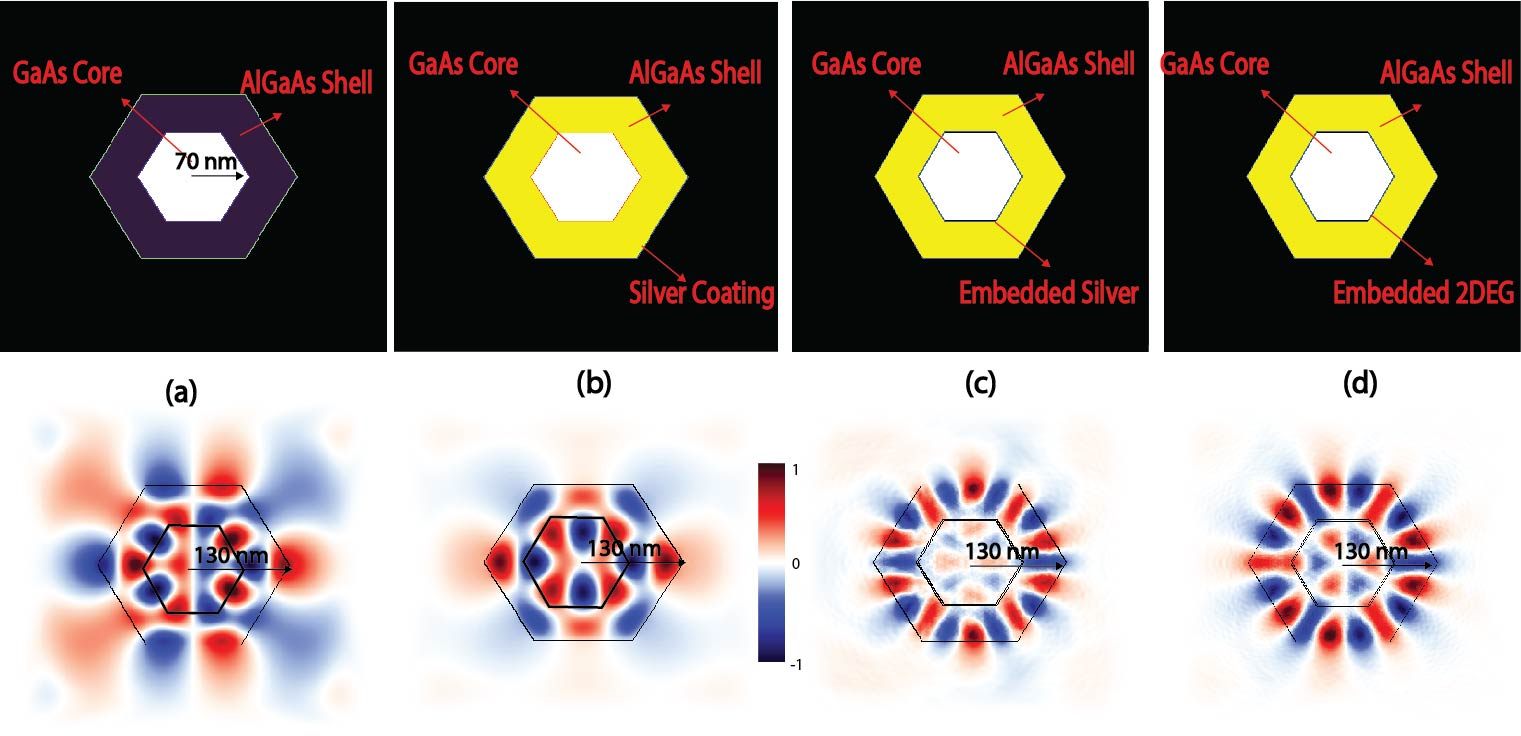
\includegraphics[width=\textwidth]{pictures/Conclusion/PlasmonMode}
  \label{PlasmonMode}
\end{figure}

Figure~\ref{PlasmonMode} shows the FDTD-simulated electric field profile (linear scale) in the
transverse plane of (a) CSNW; (b) CSNW with silver coating; (c) CSNW with and
embedded silver layer between the core and the shell; (d) CSNW with 2DEG at the
hetero-interface. As shown in Fig, coating the wire with metal introduces
plasmonic modes in the structure that enhance light confinement. Metal embedded
betweeen the core and the shell has similar effect. Importantly, we observe
that similar plasmonic features can be obtained due to the 2DEG that is
embedded in CSNW~\cite{montazeri2016plasmonic}.

Recently, the analysis of big data has become the engine for societal,
financial, scientific, and technological endeavors. This demands an
infrastructure that is capable of fast and reliable high volume data
processing. Traditionally, this requirement was fulfilled by silicon
technology. However, silicon-based technology has its own limitations, such as
speed limit and heat dissipation problem. In order to process high volume data,
we need data computation, storage, and communication to work in concert as the
three fundamental functions of a computation cell. As schematically shown in
Fig.~\ref{NWPIC_NB}, a monolithic nanosystem may be envisioned, which
incorporates NWs as waveguides, detectors, photovoltaic cells, antennas,
modulators, (photo)capacitors, LEDs and lasers. These components may be
incorporated in circuit layers, such as network-on-chip. Different layers can
communicate using NW through-silicon vias (TSVs). Similar
low-power/high-performance advantags can be realized through achievement of
high interconnect densities on the 2.5D through-Si-interposer (TSI) as reported
in reference~\cite{Zhang:2015ec} 

\begin{figure}
  \caption{Schematic depiction of an optoelectronic nanosystem may include key components such as NW LED/laser source, photodetector/photocapacitor, NW antennas, and NW-enabled network-on-chip integrated on silicon.}
  \centering
  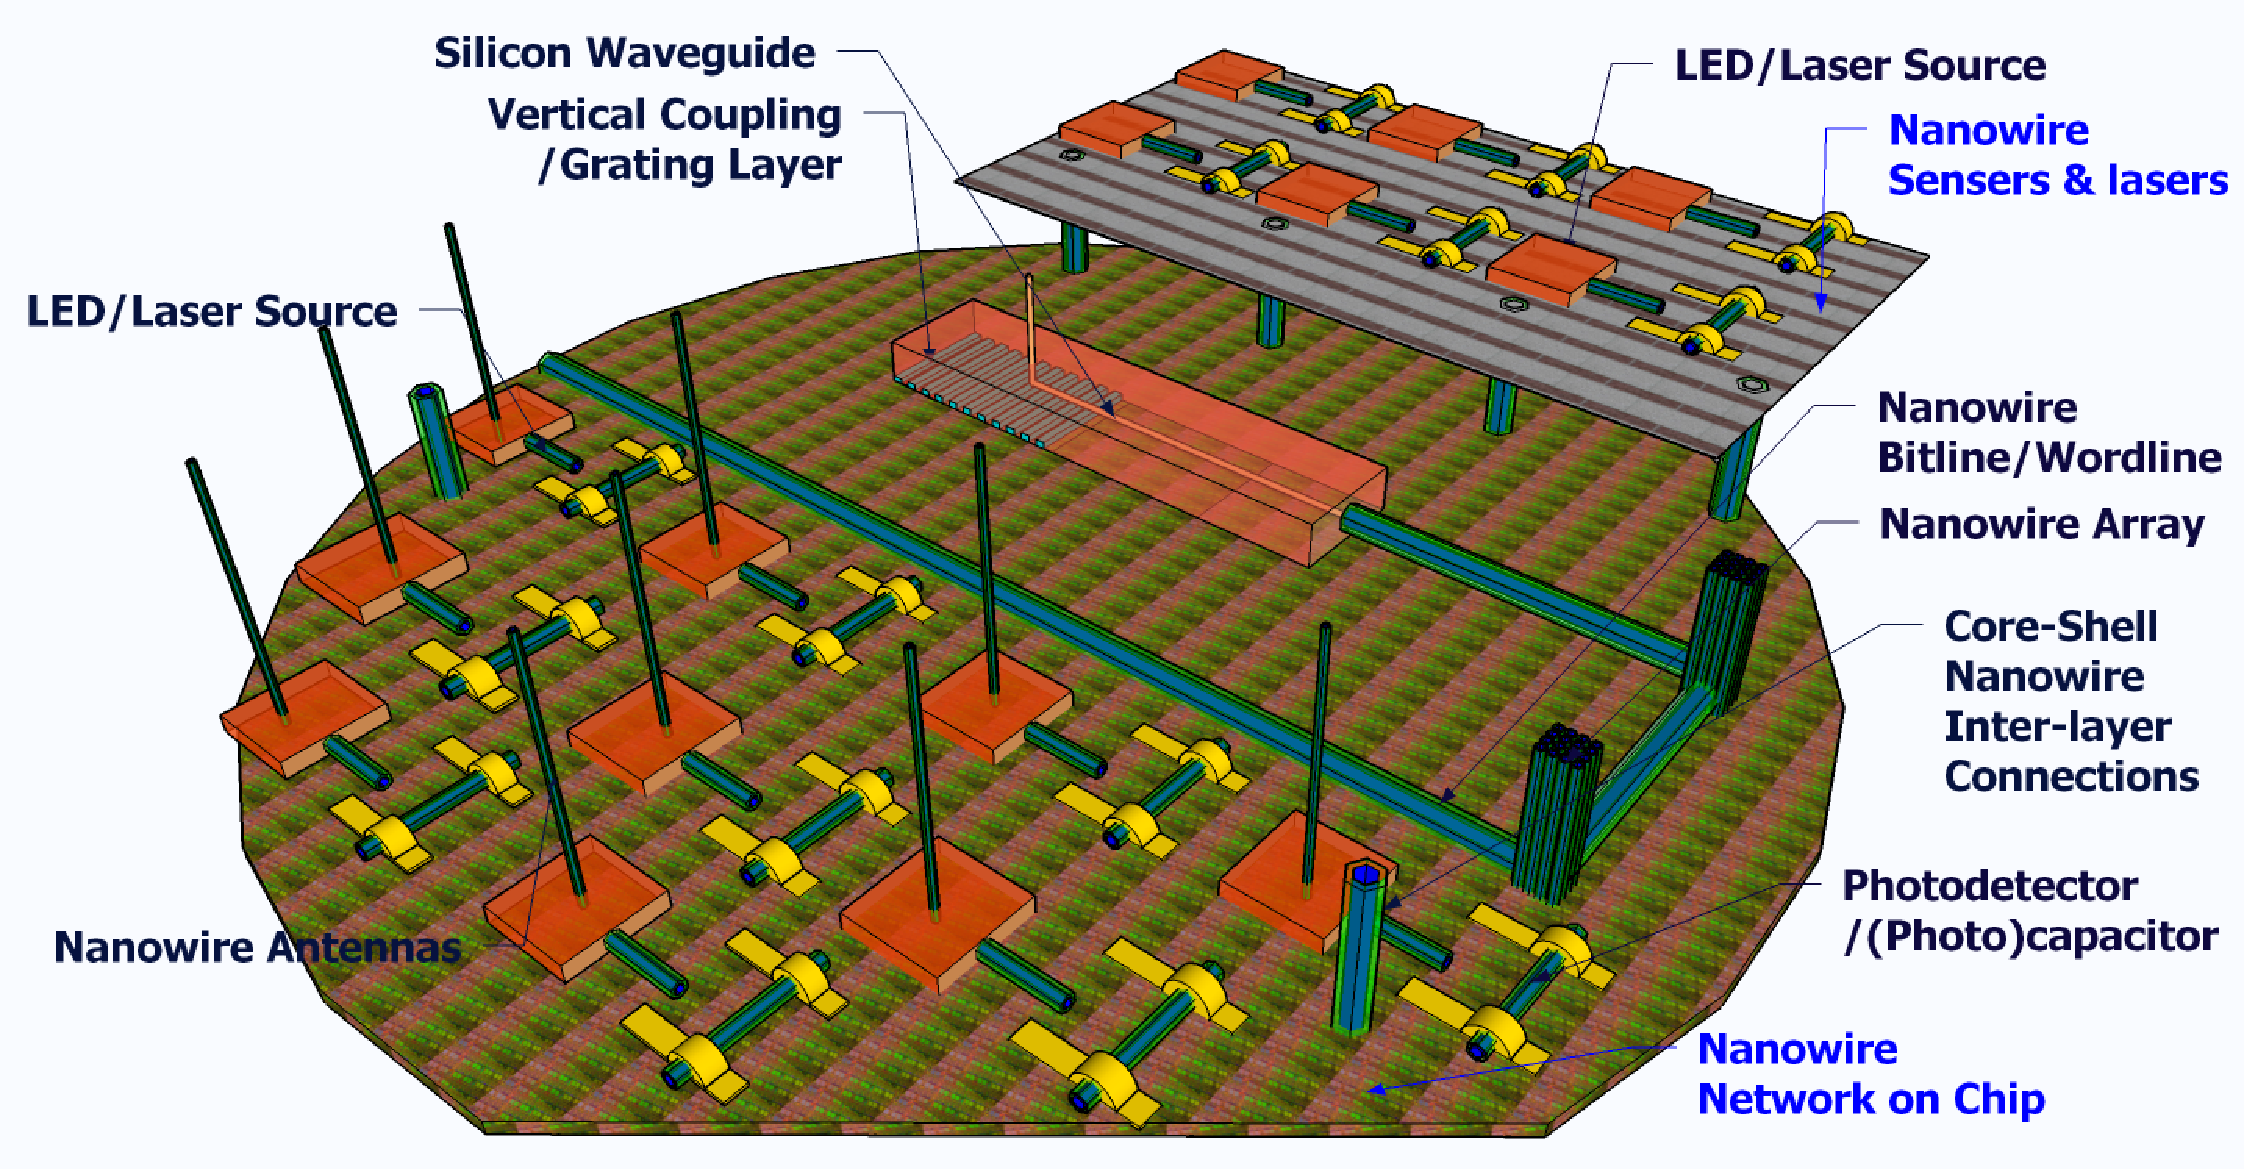
\includegraphics[width=\textwidth]{pictures/Conclusion/NWPIC_NB}
  \label{NWPIC_NB}
\end{figure}
%In Chapter~\ref{data} we brought together data from the mid-IR through the UV
%for the purpose of creating multi-wavelength SEDs for the SDSS DR7 quasars
%catalog.  This involved cross-matching mid-IR data from {\em Spitzer} and {\em
%WISE}, near-IR data from 2MASS and UKIDSS, and UV data from {\em GALEX}.  From
%this cross matched data set we created several subsets used throughout our
%studies.  We began with a (observationally) non-reddened data set used to
%explore trends in the SEDs based on various observed properties. To study the
%dust reddening properties of our quasars we limited our data to quasars
%uniformly selected by the SDSS quasar detection pipeline.  This data set was
%further split into quasar with BALs and quasars without BALs.  Finally, when
%exploring our SEDs as function of $\mbh$ we further limited this sample to the
%non-BAL quasars since BALs can make the estimated values for $\mbh$ invalid.

